% ex: ts=2 sw=2 sts=2 et filetype=tex
% SPDX-License-Identifier: CC-BY-SA-4.0

\section{Introducción e instalación}

\begin{frame}[c]{¿Qué es Matplotlib?}
  \begin{itemize}
    \item Matplotlib es una biblioteca de trazado de gráficos de bajo
          nivel en Python que sirve como utilidad de visualización.
    \pausa
    \item Matplotlib fue creado por John D. Hunter.
    \pausa
    \item Matplotlib es de código abierto y podemos usarlo libremente.
    \pausa
    \item Matplotlib está escrito principalmente en Python, algunos
          segmentos están escritos en C, Objective-C y Javascript
          para compatibilidad con la plataforma.
  \end{itemize}
\end{frame}

\begin{frame}[c]{¿Dónde está el código base de Matplotlib?}
  \begin{itemize}
    \item El código fuente de Matplotlib se encuentra en este
      repositorio de github
      \href{https://github.com/matplotlib/matplotlib}
      {https://github.com/matplotlib/matplotlib}
  \end{itemize}
\end{frame}

\begin{frame}[fragile]
  \frametitle{Instalación de Matplotlib}
    Si ya tiene Python y PIP instalados en un sistema,
    entonces la instalación de Matplotlib es muy fácil.

  \begin{exampleblock}{Ejemplo:}
    Instálalo usando este comando:
    \begin{lstlisting}[language=Python]
C:\Users\Your Name>pip install matplotlib 
    \end{lstlisting}
  \end{exampleblock}
  Si este comando falla, utilice una distribución de Python que
  ya tenga Matplotlib instalado, como Anaconda, Spyder, etc.
\end{frame}

\begin{frame}[fragile]
  \frametitle{Importar Matplotlib}
    Una vez instalado Matplotlib, impórtelo en sus aplicaciones
    agregando la declaración: \textbf{import module}
  \begin{exampleblock}{Ejemplo:}
    \begin{lstlisting}[language=Python]
import matplotlib
    \end{lstlisting}
  \end{exampleblock}
  Ahora Matplotlib está importado y listo para usar
\end{frame}

\begin{frame}[fragile]
  \frametitle{Comprobación de la versión de Matplotlib}

  La cadena de versión se almacena en \textbf{\_\_version\_\_} el atributo.

  \begin{exampleblock}{Ejemplo:}
    \begin{lstlisting}[language=Python]
import matplotlib

print(matplotlib.__version__)
    \end{lstlisting}
  \end{exampleblock}
  \begin{block}{Nota:}
    Se utilizan dos caracteres de subrayado en \textbf{\_\_version\_\_}.
  \end{block}
\end{frame}

\section{Gráficos con Pyplot}

\begin{frame}[fragile]
  \frametitle{Pyplot}

  La mayoría de las utilidades de Matplotlib se encuentran
  bajo el submódulo \textbf{pyplot} y normalmente se importan
  bajo el alias \textbf{plt}:

  \begin{exampleblock}{Ejemplo:}
    \begin{lstlisting}[language=Python]
import matplotlib.pyplot as plt 
    \end{lstlisting}
  \end{exampleblock}
  Ahora el paquete Pyplot puede denominarse plt.
\end{frame}

\begin{frame}[fragile]
  \frametitle{Pyplot}

  \begin{columns}
      \column{0.5\textwidth}
        \begin{exampleblock}{Ejemplo:}
          Dibuje una línea en un diagrama desde la posición
          (0,0) hasta la posición (6,250):
          \lstinputlisting{ejemplos/e01.py}
        \end{exampleblock}
      \column{0.5\textwidth}
      \pausa
      \begin{center}
          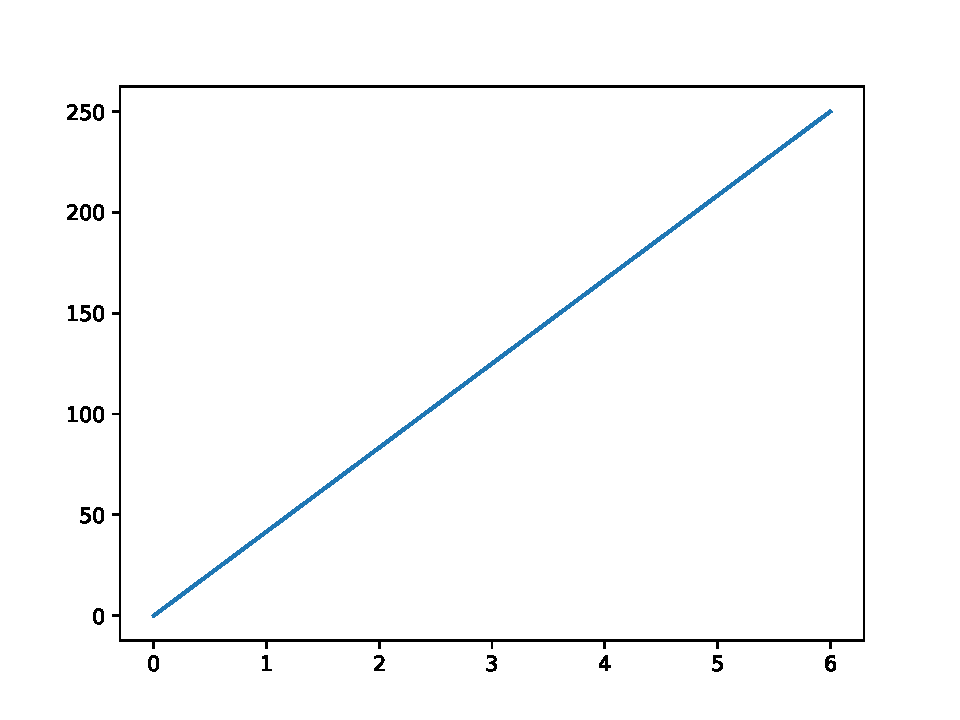
\includegraphics[scale=0.5]{ejemplos/e01.pdf}
      \end{center}
  \end{columns}
\end{frame}

\begin{frame}[c]{Graficando los puntos "x" y "y"}
  \begin{itemize}
    \item La función \textbf{plot()} se utiliza para dibujar puntos
      (marcadores) en un diagrama.
    \pausa
    \item De forma predeterminada, la función \textbf{plot()} dibuja
      una línea de un punto a otro.
    \pausa
    \item La función toma parámetros para especificar puntos en el diagrama.
    \pausa
    \item El parámetro 1 es una matriz que contiene los puntos en el
      \textbf{eje x}.
    \pausa
    \item El parámetro 2 es una matriz que contiene los puntos en el
      \textbf{eje y}.
    \pausa
    \item Si necesitamos trazar una línea desde (1, 3) a (8, 10),
      tenemos que pasar dos matrices [1, 8] y [3, 10] a la función de trazado.
  \end{itemize}
\end{frame}

\begin{frame}[fragile]
  \frametitle{Graficando los puntos "x" y "y"}

  \begin{columns}
      \column{0.5\textwidth}
        \begin{exampleblock}{Ejemplo:}
          Se dibuja una línea en un diagrama desde la posición
          (1, 3) a la posición (8, 10):
          \lstinputlisting{ejemplos/e02.py}
        \end{exampleblock}
      \column{0.5\textwidth}
      \pausa
      \begin{center}
          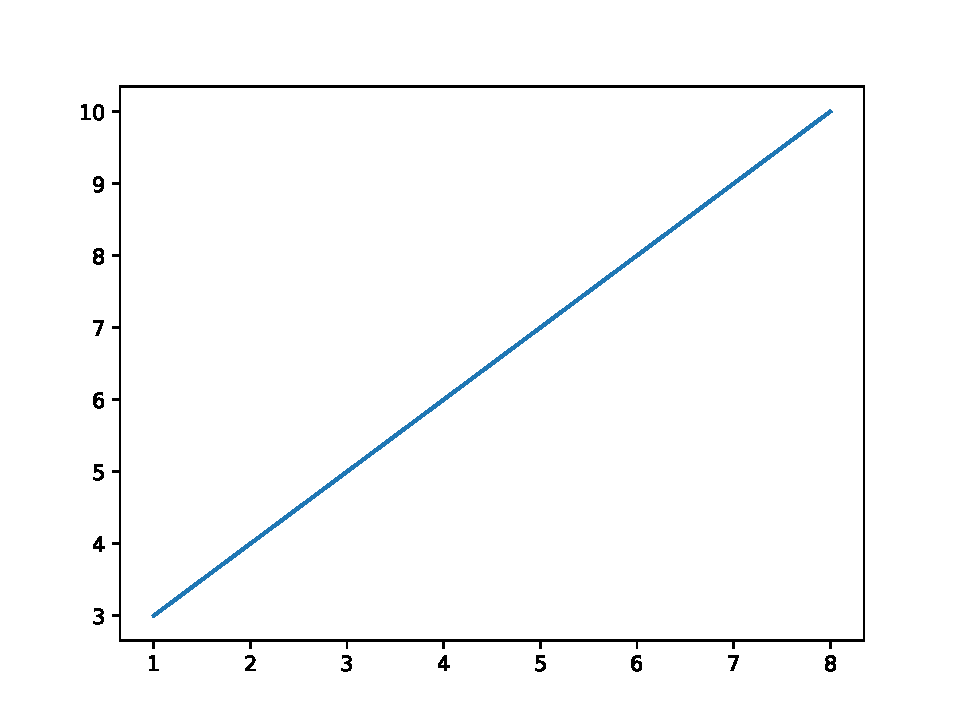
\includegraphics[scale=0.4]{ejemplos/e02.pdf}
      \end{center}
      \begin{itemize}
        \item El eje x es el eje horizontal.
        \item El eje y es el eje vertical.
      \end{itemize}
  \end{columns}
\end{frame}

\begin{frame}[fragile]
  \frametitle{Trazando sin línea}

  \vspace{\baselineskip}
  Para trazar solo los marcadores, puede utilizar el parámetro
  de notación de cadena de acceso directo "o", que significa "anillos".
  \begin{columns}
      \column{0.5\textwidth}
        \begin{exampleblock}{Ejemplo:}
          Dibuje dos puntos en el diagrama, uno en la
          posición (1, 3) y otro en la posición (8, 10):
          \lstinputlisting{ejemplos/e03.py}
        \end{exampleblock}
      \column{0.5\textwidth}
      \pausa
      \parbox{\textwidth}{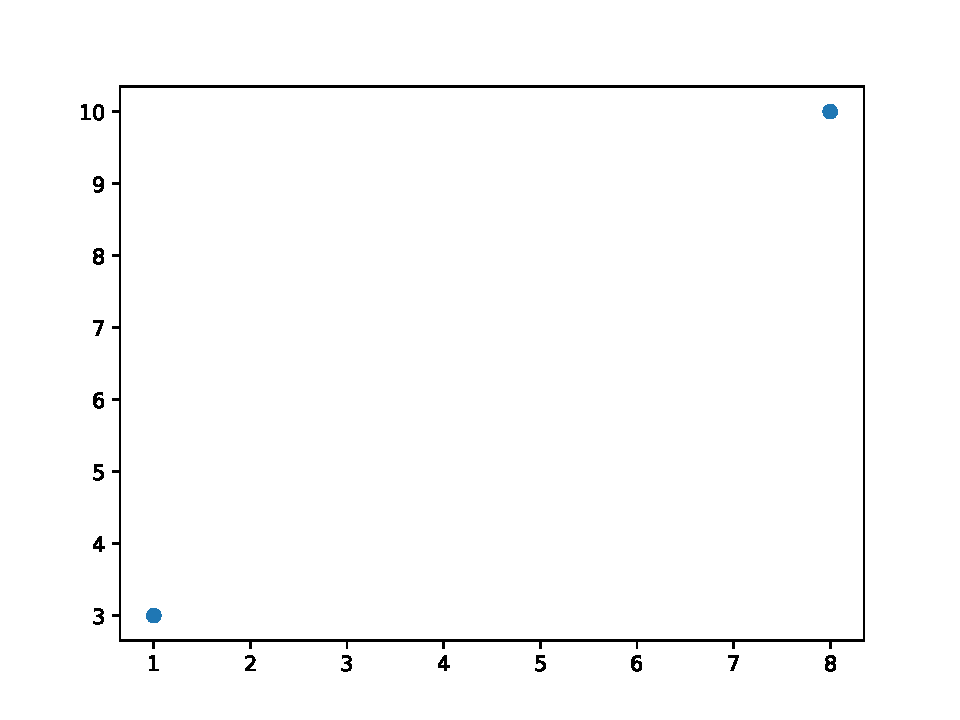
\includegraphics[width=\linewidth]{ejemplos/e03.pdf}}
  \end{columns}
\end{frame}

\begin{frame}[fragile]
  \frametitle{Puntos múltiples}

  \vspace{\baselineskip}
  Puedes trazar tantos puntos como desees, sólo asegúrate de
  tener la misma cantidad de puntos en ambos ejes.
  \begin{columns}
      \column{0.5\textwidth}
        \begin{exampleblock}{Ejemplo:}
          Dibuje una línea en un diagrama desde la posición
          (1, 3) a (2, 8), luego a (6, 1) y finalmente a
          la posición (8, 10):
          \lstinputlisting{ejemplos/e04.py}
        \end{exampleblock}
      \column{0.5\textwidth}
      \pausa
      \parbox{\textwidth}{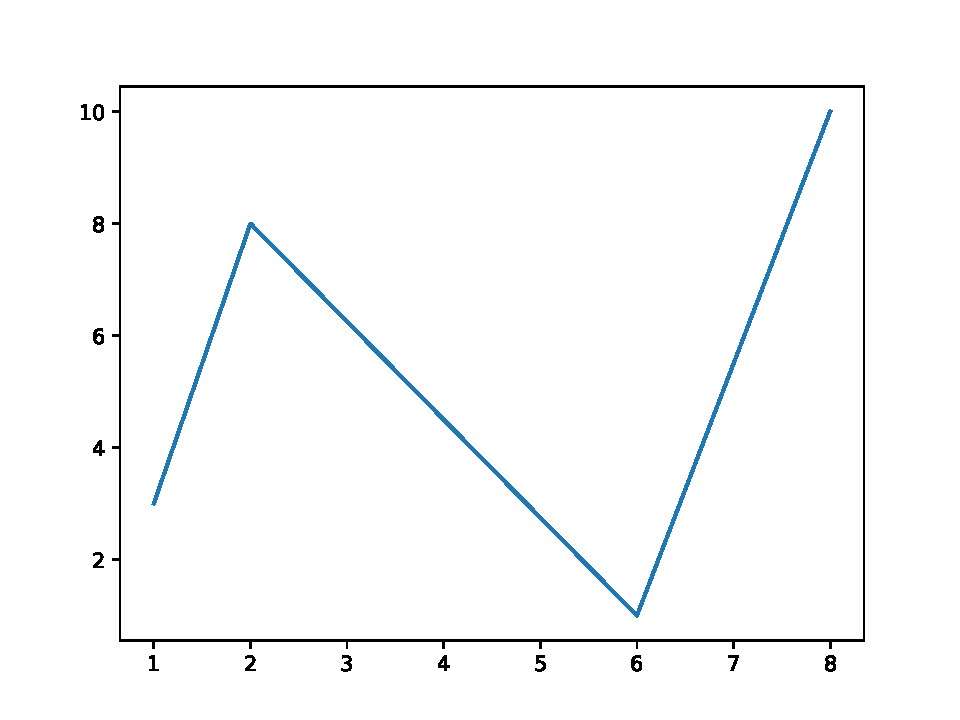
\includegraphics[width=\linewidth]{ejemplos/e04.pdf}}
  \end{columns}
\end{frame}

\begin{frame}[fragile]
  \frametitle{Puntos X predeterminados}

  \vspace{\baselineskip}
  Si no especificamos los puntos en el eje x, obtendrán los
  valores predeterminados 0, 1, 2, 3, etc., dependiendo de la
  longitud de los puntos y.

  Entonces, si tomamos el mismo ejemplo anterior y omitimos los
  puntos x, el diagrama se verá así:
  \begin{columns}
      \column{0.6\textwidth}
        \begin{exampleblock}{Ejemplo:}
          Trazando sin puntos x:
          \lstinputlisting{ejemplos/e05.py}
        \end{exampleblock}
      \column{0.4\textwidth}
      \pausa
      \parbox{\textwidth}{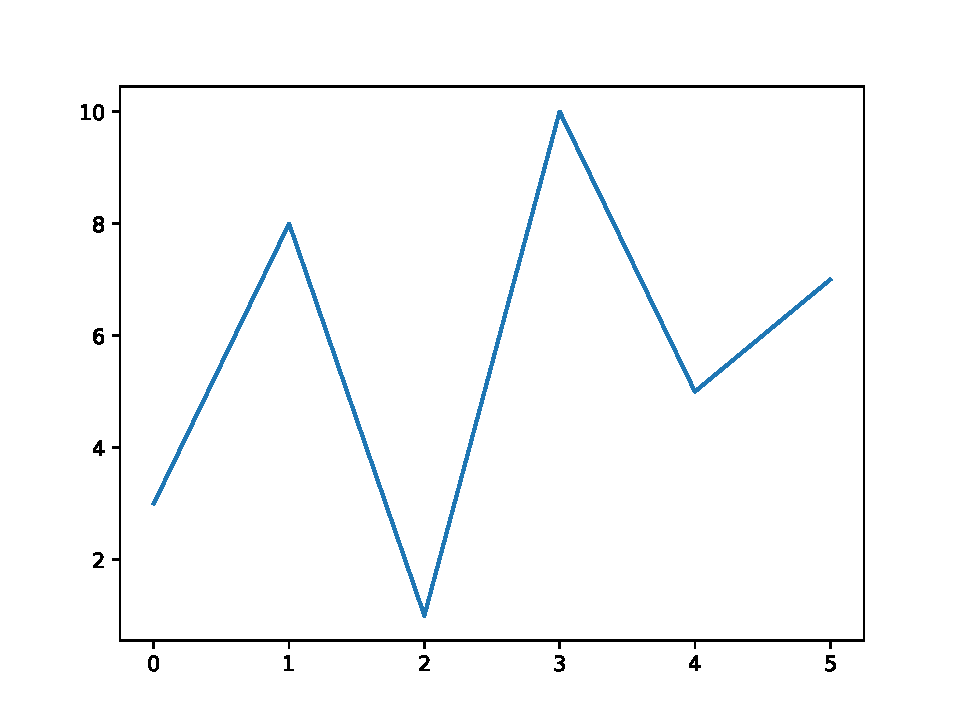
\includegraphics[width=55mm]{ejemplos/e05.pdf}}
      \begin{itemize}
        \item Los puntos x en el ejemplo son [0, 1, 2, 3, 4, 5].
      \end{itemize}
  \end{columns}
\end{frame}

\section{Gráfica de barras}

\begin{frame}[fragile]
  \frametitle{Creación de barras}

  \vspace{\baselineskip}
  Con Pyplot, puedes utilizar la función \textbf{bar()}
  para dibujar gráficos de barras:
  \begin{columns}
      \column{0.5\textwidth}
        \begin{exampleblock}{Ejemplo:}
          Dibuja 4 barras:
          \lstinputlisting{ejemplos/e06.py}
        \end{exampleblock}
      \column{0.5\textwidth}
      \pausa
      \parbox{\textwidth}{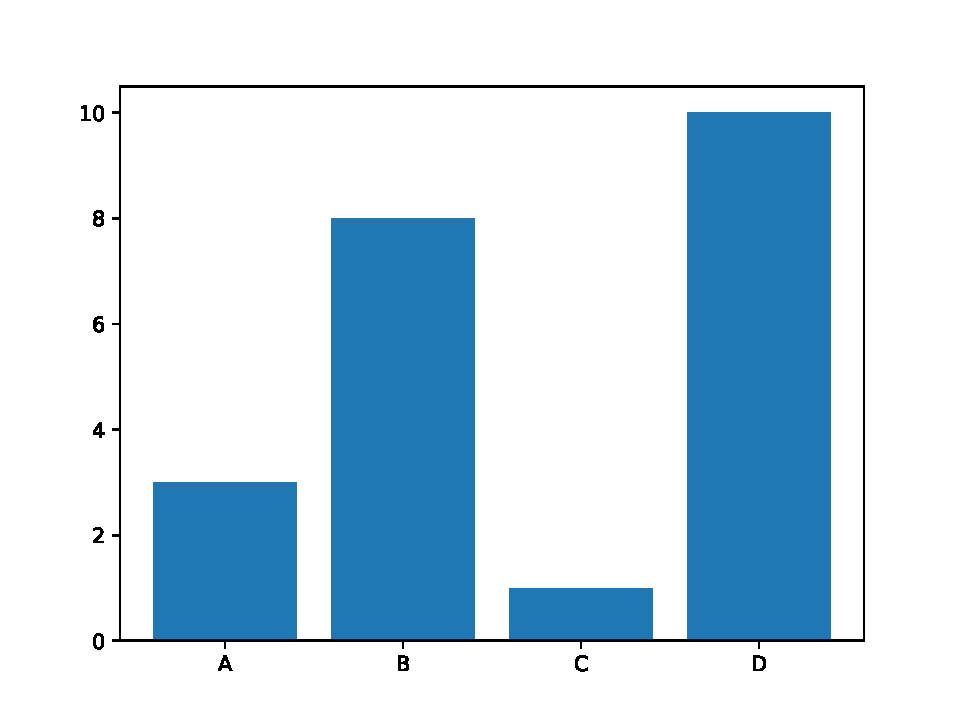
\includegraphics[width=\linewidth]{ejemplos/e06.pdf}}
  \end{columns}
\end{frame}

\begin{frame}[fragile]
  \frametitle{Creación de barras}

  \vspace{\baselineskip}
  La función \textbf{bar()} toma argumentos que describen
  el diseño de las barras.

  Las categorías y sus valores representados por el primer
  y segundo argumento como matrices.
  \begin{columns}
      \column{0.5\textwidth}
        \begin{exampleblock}{Ejemplo:}
          Dibuja 4 barras:
          \lstinputlisting{ejemplos/e07.py}
        \end{exampleblock}
      \column{0.5\textwidth}
      \pausa
      \parbox{\textwidth}{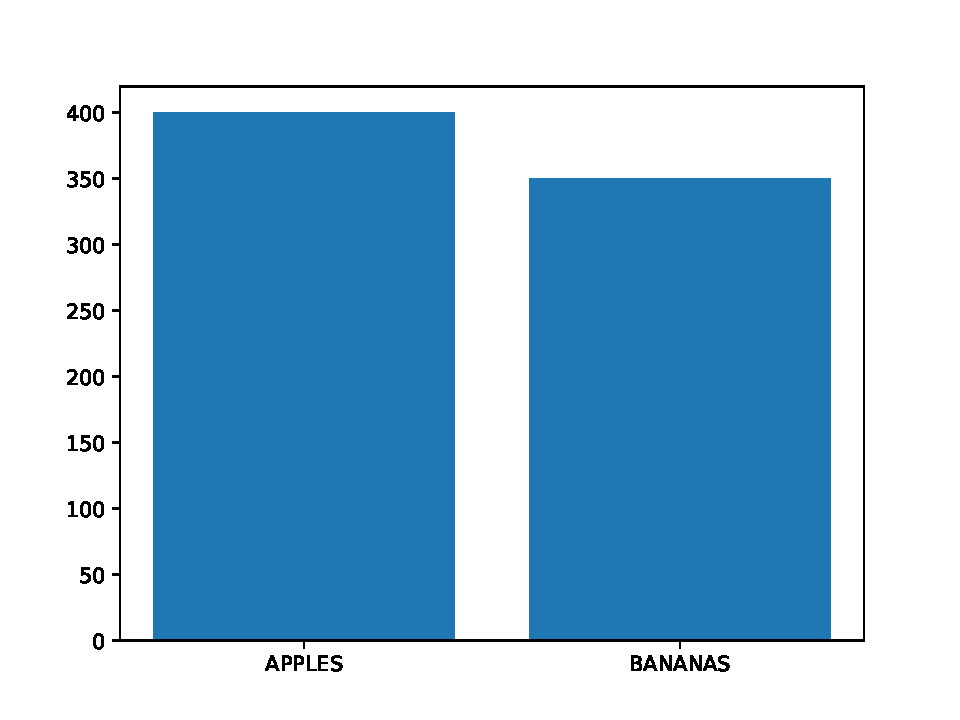
\includegraphics[width=\linewidth]{ejemplos/e07.pdf}}
  \end{columns}
\end{frame}

\begin{frame}[fragile]
  \frametitle{Barras horizontales}

  \vspace{\baselineskip}
  Si desea que las barras se muestren horizontalmente
  en lugar de verticalmente, utilice la función \textbf{barh()}:
  \begin{columns}
      \column{0.5\textwidth}
        \begin{exampleblock}{Ejemplo:}
          \lstinputlisting{ejemplos/e08.py}
        \end{exampleblock}
      \column{0.5\textwidth}
      \pausa
      \parbox{\textwidth}{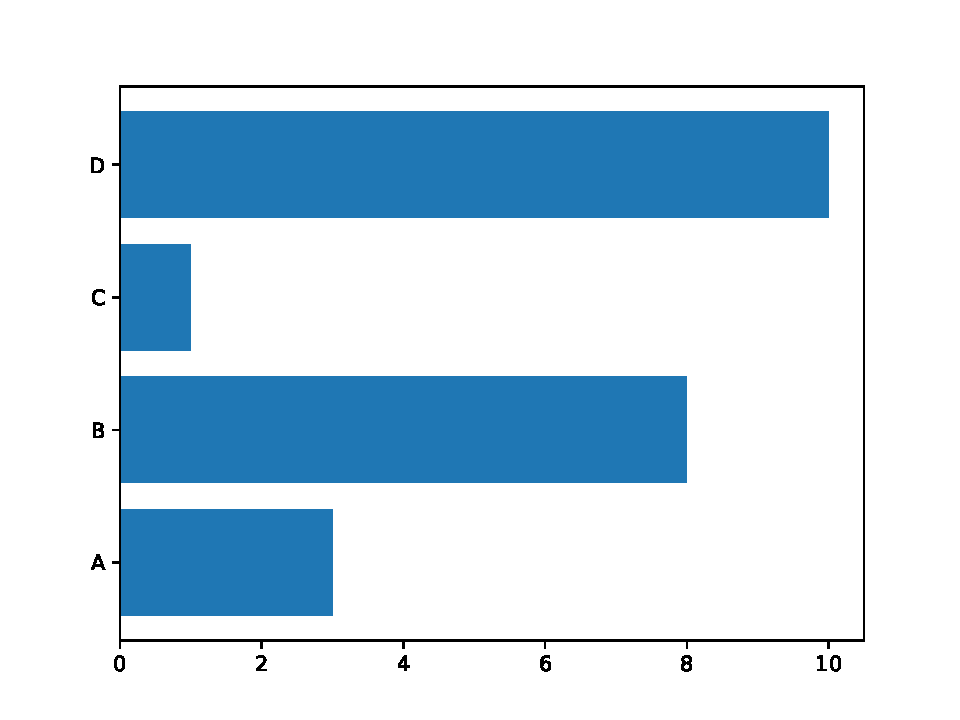
\includegraphics[width=\linewidth]{ejemplos/e08.pdf}}
  \end{columns}
\end{frame}

\begin{frame}[fragile]
  \frametitle{}
  \begin{columns}
      \column{0.5\textwidth}
        \begin{exampleblock}{Ejemplo:}
          \lstinputlisting{ejemplos/e02.py}
        \end{exampleblock}
      \column{0.5\textwidth}
      \pausa
      \begin{center}
          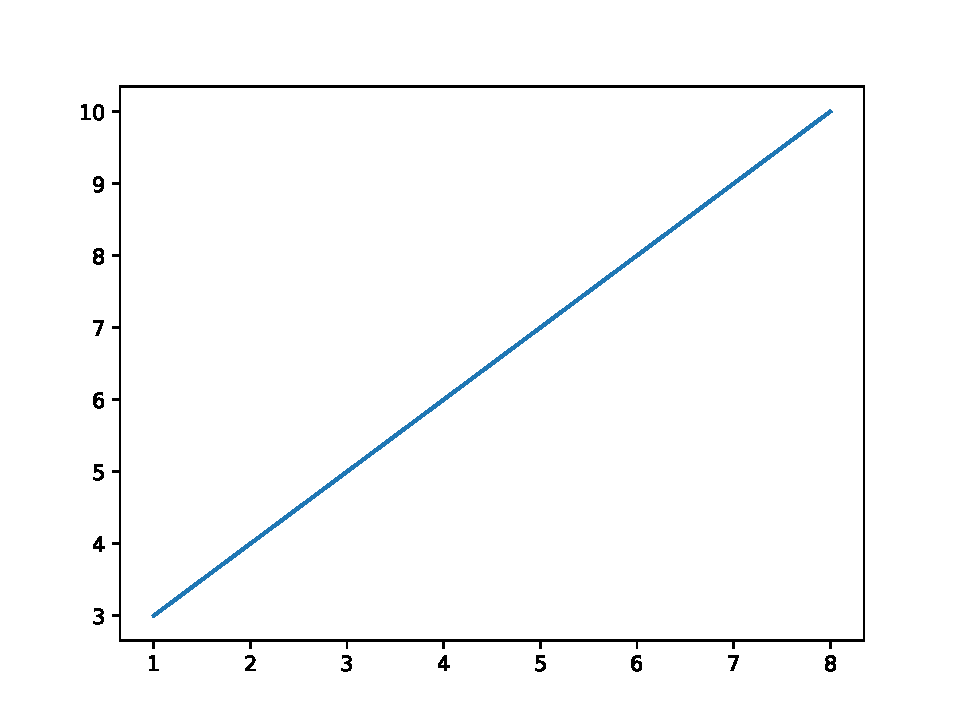
\includegraphics[scale=0.4]{ejemplos/e02.pdf}
      \end{center}
      \begin{itemize}
        \item 
      \end{itemize}
  \end{columns}
\end{frame}

\begin{frame}[fragile]
  \frametitle{}

  \begin{exampleblock}{Ejemplo:}
    \begin{lstlisting}[language=Python]
    \end{lstlisting}
  \end{exampleblock}
\end{frame}
